\documentclass[a4paper,twoside,openany]{book}
%twoside Specifies whether double or single sided output should be generated.
%openright/openany Makes chapters begin either only on right hand pages or on the next page available.
\usepackage{geometry}
\geometry{a4paper,top=3cm,bottom=3cm,left=3cm,right=3cm,heightrounded,bindingoffset=1cm}


\usepackage[italian, english]{babel}
\usepackage[T1]{fontenc}
\usepackage{lmodern}
\usepackage{color}
\usepackage{float}
\usepackage{graphicx}
\usepackage{amssymb}
\usepackage{amsmath}
\everymath{\displaystyle}
\usepackage{cancel}
\usepackage{booktabs}
\usepackage{multirow}
\usepackage{siunitx}
\usepackage{subcaption}
\usepackage{hyperref}
\usepackage{hyphenat}
\usepackage{verbatim}
\usepackage{chemformula}
\usepackage{color}
\definecolor{maroon(html/css)}{rgb}{0.5, 0.0, 0.0}
\usepackage{nicematrix}
\usepackage{rotating}

\begin{document}
	\begin{titlepage}
		\centering
		
\includegraphics[width=0.3\textwidth]{university}\\
		\bigskip
		{\Large
		{\scshape Università degli Studi di Milano Bicocca}\\
		{\scshape Dipartimento di Fisica}\\
		{\scshape "Giuseppe Occhialini"}\\
		\bigskip
		{\scshape Corso di Laurea Magistrale in Fisica}\\}
		Anno Accademico 2024/2025\\
		\bigskip
		{\hfill\vfill{\scshape \Huge{\textcolor{maroon(html/css)}{Characterization of a Lanthanum Bromide crystal}}}\\}
		{\vfill
		\[	\begin{array}{c}
			\mbox{Andrea Baiocco}\\
			\mbox{Giovanni Locatelli}\\
			\mbox{Gabriele Papasodaro}\\
			\mbox{Alberto Sala}
			\end{array}	\]}
	\end{titlepage}

\newpage
\null
\thispagestyle{empty}
\newpage

\pagenumbering{Roman}
\setcounter{page}{1}
\begin{center}\textbf{Summary}\\\end{center}
The experience's aim is to characterize the detection efficiency of a Lanthanum Brumide ($\ch{LaBr3}$) scintillator crystal by studying its intrinsic radioactivity through the decay of $^{138}\ch{La}$.  Then starting from this results, we want to identify an unknown radioactive source and estimate the activity of a radioactive source of Cesium ($^{137}\ch{Cs}$).\\

The design of the machine is describe as show in figure \ref{strum}

\begin{figure}[H]
\centering
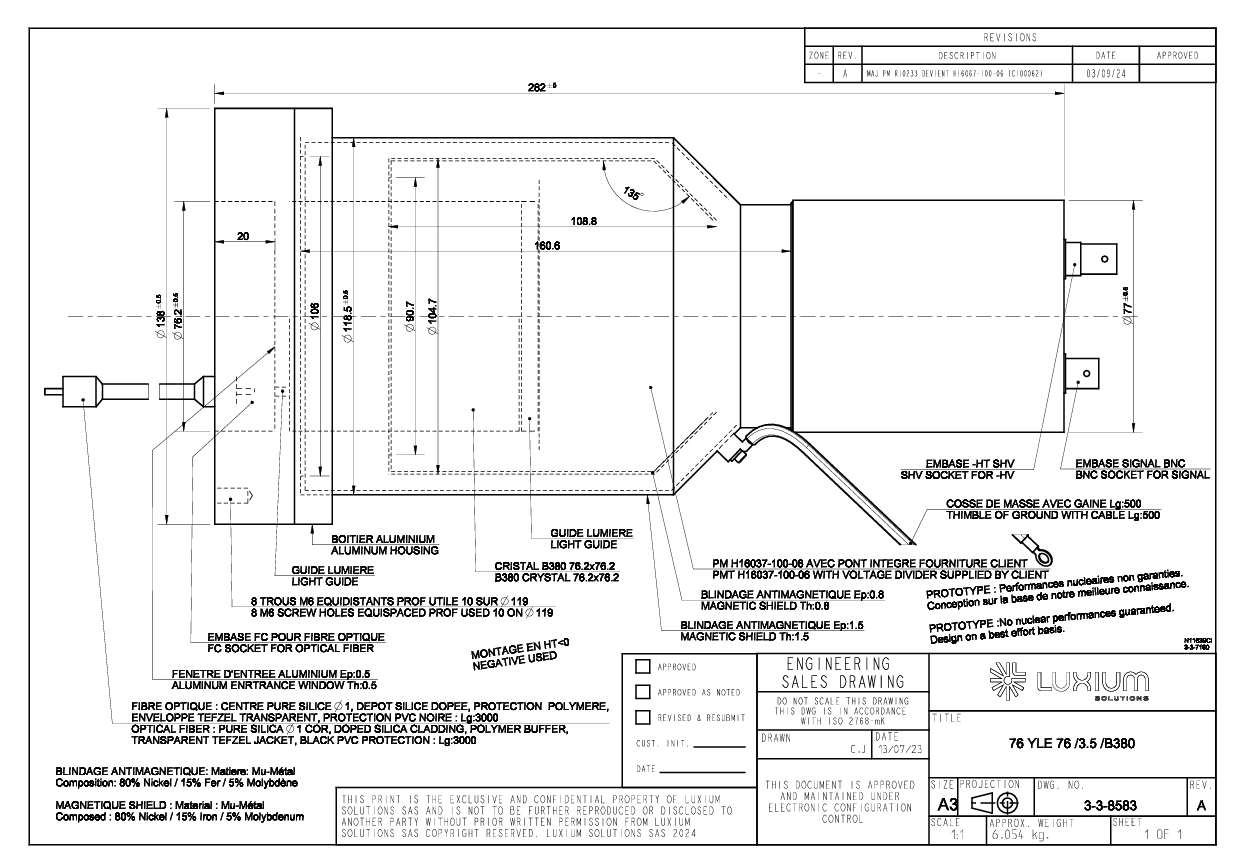
\includegraphics[width=0.5\textwidth]{Strumento}
\caption{Design instrument}
\label{strum}
\end{figure}

\newpage
\null
\thispagestyle{empty}
\newpage

\pagenumbering{Roman}
\setcounter{page}{1}
\tableofcontents

\newpage
\null
\thispagestyle{empty}
\newpage

\pagenumbering{arabic}
\setcounter{page}{1}
\chapter{Instruments description}
	\section {Tools list}
\begin{itemize}
\item Phototube with scintillator crystal $\ch{La}(:\ch{Ce}\,5\%)\ch{Br3}$
\item some radioactive source as $^{137}\ch{Cs}$, $^{22}\ch{Na}$ and an unknown source
\item voltage generator
\item PhotoMultiplier Tube (PMT)
\item BNC connections
\item digitizer
\item plates and supports of different sizes
\end{itemize}

	\section{PMT and scintillator crystal}
The operation of a scintillator crystal is based on the process of radiation-matter interaction and its purpose is to transform the signal given by a photon into a measurable electrical signal. Following the interaction with an incident photon, an electron of the crystal is released, losing energy and exciting the electrons of the semiconductor, taking them from the valence band to the conduction band. 

These, de-excited, emit an optical photon that cannot be absorbed by the semiconductor because it is doped. This photon produces, by photoelectric effect on the photocathode, an electron that is amplified inside a photomultiplier by a series of dynodes placed at different potentials, guaranteeing a gain of $10^{5}$ or $10^{6}$ electrons.

In our case, a crystal of Lanthanum Bromide doped at $5\%$ with Cerium was used. Lanthanum Bromide contains a radioactive isotope, $^{138}\ch{La}$ (a.i $0.08881\%$) with a half-life of $1.03  \cdot 10^{11}$ years that decays by electron capture (BR $65.2\%$) on an excited state of $^{138}\ch{Ba}$. When de-excited, it emits a $\gamma$ beam at 1436 KeV. 

The choice of this crystal was dictated precisely by its intrinsic radioactivity which allows to obtain important information on the detection efficiency of the instrument and allows to carry out its calibration. Furthermore, thanks to the short scintillation time, the crystal allows to have a high counting rate similar to what occurs in plasmas.

	\section{Digitizer, AC generator and BNC connections}
About electrical components, in the experience we used an AC voltage generator connected via BNC cables to the instrumentation, thus powering the PMT inside the machine.

Instead, the digitalizer allows to convert the analogical signal we are evaluating into an electrical signal.

	\section{Support and plates}
The last component are support and plates of different size. They are used mainly in study of efficiency at various distances. The size of plates are 5 or 10\,cm.

\chapter{Data Analysis}
First, connect the PMT to a high-voltage generator and, since you want to polarize the photo-tube negatively, it must be connected to the negative channel of the generator, while the positive channel of the latter is zeroed via a coaxial cable (which functions as ground).

The photo-tube is then connected to an oscilloscope and, by observing how the output signal varies, the voltage to use is determined. Even at low voltages, a signal begins to appear on the oscilloscope. This is because $^{138}\ch{La}$ isotope, being radioactive, emits radiation, which, once converted into "visible" photons by the scintillator crystal, is detected by the PMT. After choosing the potential difference, equal to 1000 V.

\begin{figure}[H]
\centering
\includegraphics[width=0.4\textwidth]{Segnale}
\caption{Oscilloscope signal}
\label{signale}
\end{figure}

Note that, since the refractive coefficients of the scintillator crystal and the PMT lens differ, it is necessary to insert optical grease (whose coefficient has an intermediate value) between the two surfaces to avoid any total reflection phenomena. Looking at the real-time signal trend output from the photomultiplier tube on the oscilloscope, one notices the presence of some unexpected peaks probably due to the random arrival of a cosmic ray. Therefore, to avoid any type of external influence, the PMT was encapsulated inside the instrument and shielded by a metal cover.

We now proceed to the actual data collection: the output signal is connected to a digitizer that transforms the signal from analog (the one read on the oscilloscope) to digital. To calibrate the digitizer, we identified the three peaks of known energy, respectively: $\beta$ decay at energy 788,74 keV and the double peaks of $\epsilon$ decay at energies 1440 and 1472 keV.

\begin{figure}[H]
    \centering
    % Prima immagine
    \begin{subfigure}{0.49\textwidth}
        \centering
        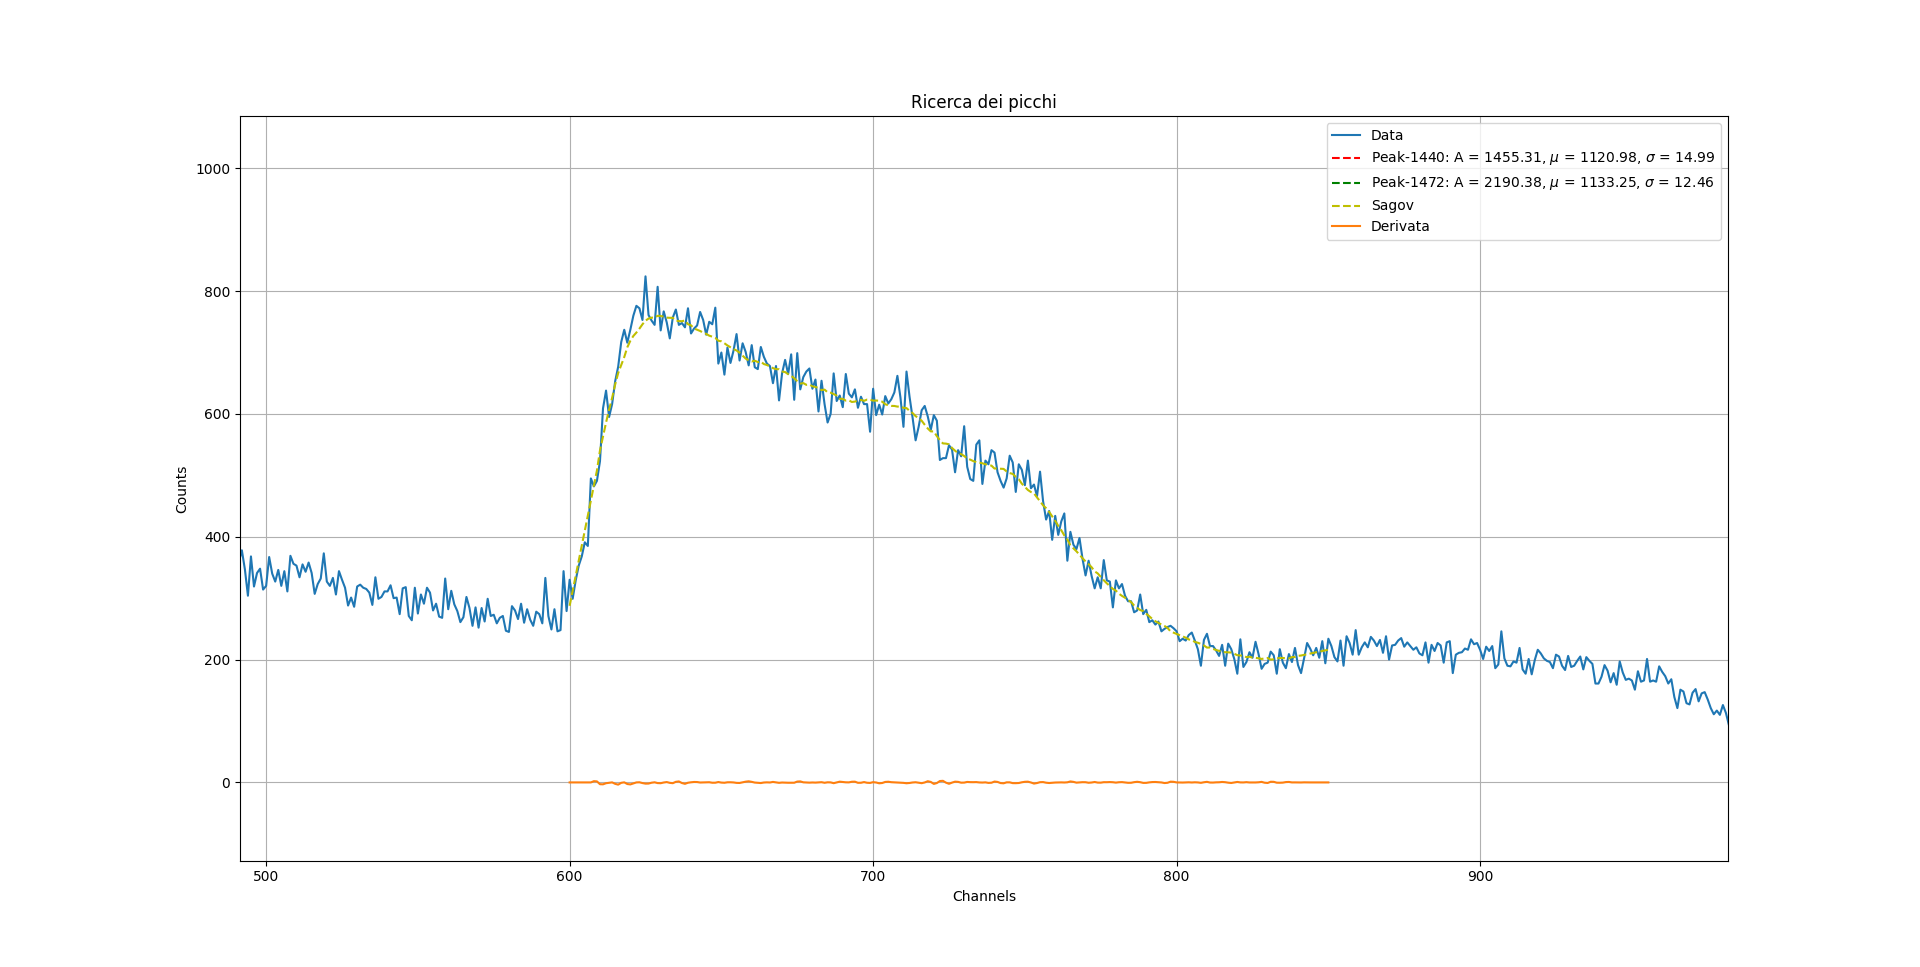
\includegraphics[width=\linewidth]{Dec_beta}
        \caption{$\beta$ decay}
        \label{bdecay}
    \end{subfigure}
    \hfill
    % Seconda immagine
    \begin{subfigure}{0.49\textwidth}
        \centering
        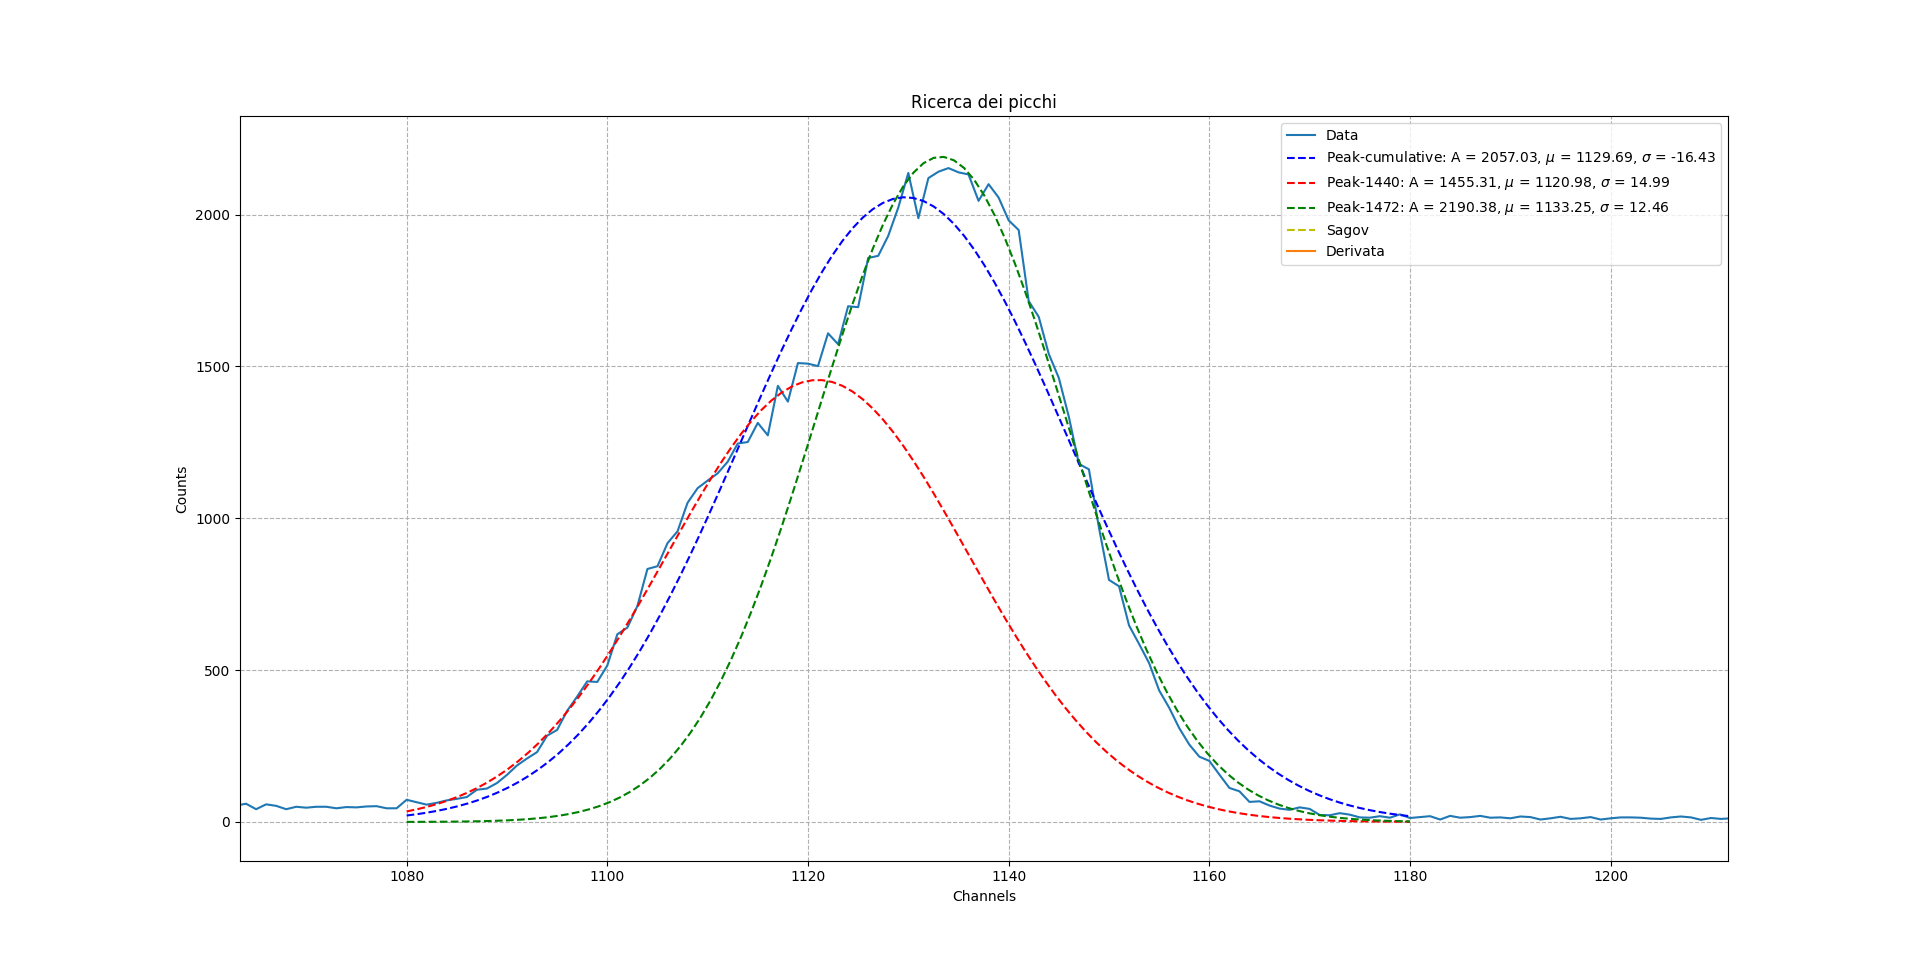
\includegraphics[width=\linewidth]{Doppia_gauss}
        \caption{$\epsilon$ decay}
        \label{edecay}
    \end{subfigure}
    \caption{Calibration peaks}
    \label{calpeaks}
\end{figure}

Finally performing a linear fit for the conversion from channels to energies, we can evaluate the calibration factor in according to the eqaution:
\begin{equation}
Energy [keV] = 1,29 \cdot Channel [Ch] + 4,47
\end{equation}

\begin{figure}[H]
\centering
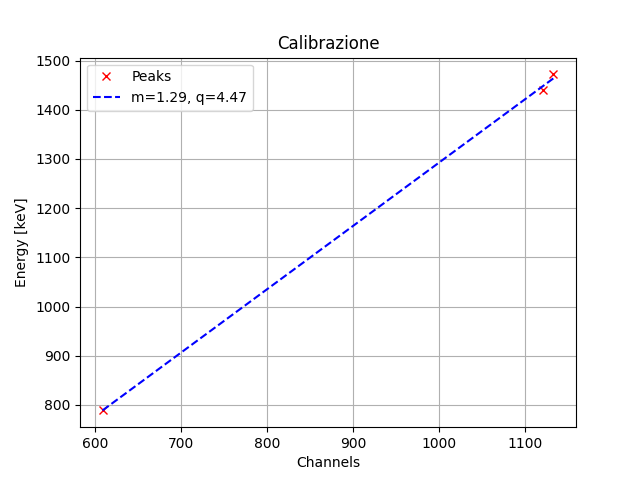
\includegraphics[width=0.7\textwidth]{Calibrazione}
\caption{Calibration}
\label{Calibration}
\end{figure}

Once the data needed to calibrate the crystal have been collected, the measurement can begin: after aligning the crystal and the cesium gel disk that will constitute the radioactive source on a workbench and verifying that the source and instrument are aligned with each other, data on the decay of the cesium are collected at various distances from the detector. In the two different cases analyzed (300 1mm and 152 1mm), it was necessary to lower the threshold to make the peak recognizable.

	\section{\ch{LaBr3} scintillator}
		\subsection{Intrinsic radioactivity}

\begin{figure}[H]
\centering
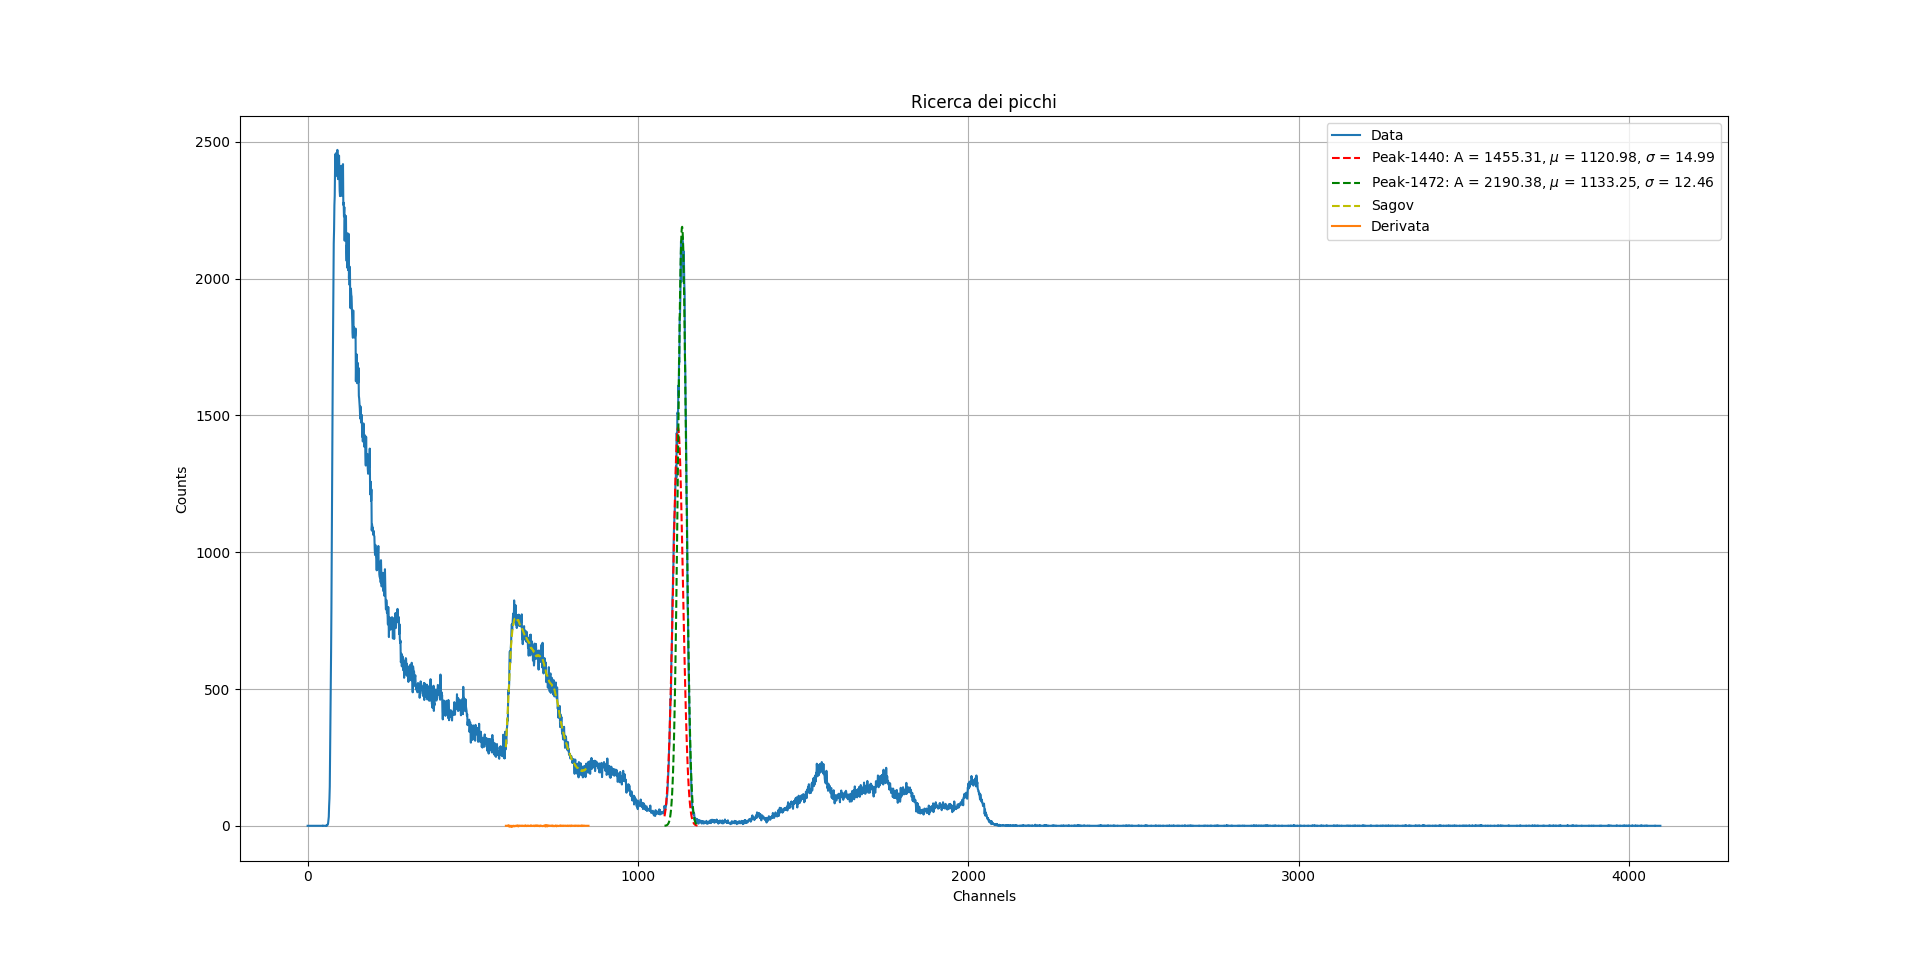
\includegraphics[width=1\textwidth]{Fondo}
\caption{Background}
\label{Fondo}
\end{figure}

\begin{figure}[H]
\centering
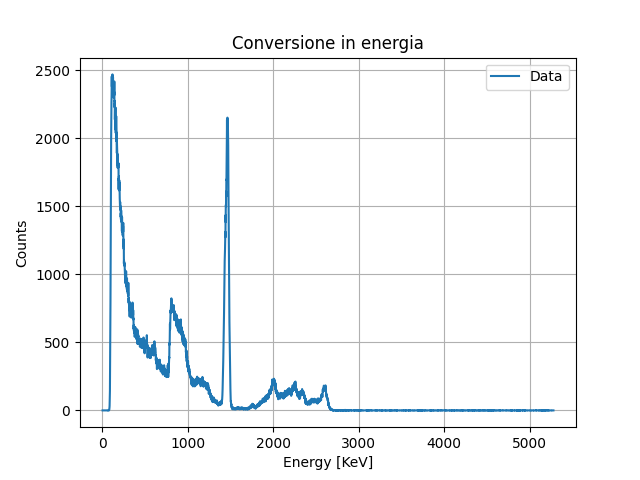
\includegraphics[width=0.5\textwidth]{Energy_conv_fondo}
\caption{Background converted}
\label{Fondo_conv}
\end{figure}

	\subsection{Detection efficiency}

\begin{figure}[H]
\centering
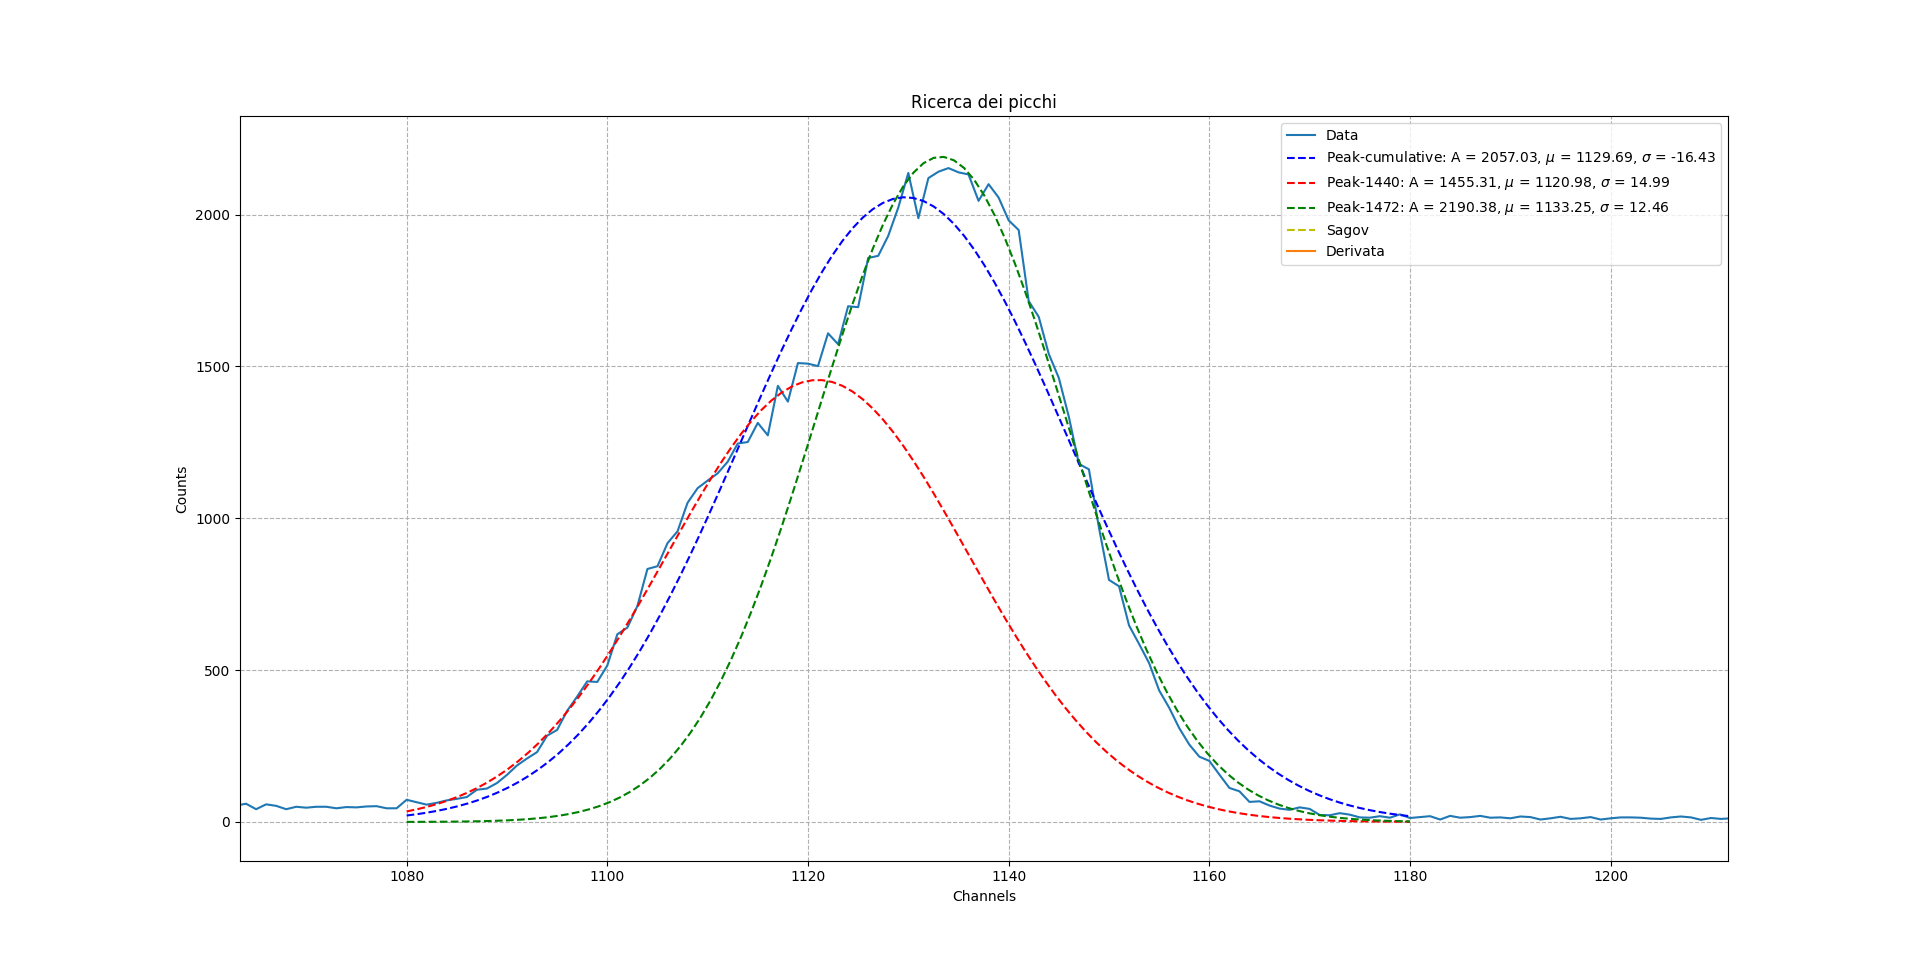
\includegraphics[width=0.7\textwidth]{Doppia_gauss}
\caption{Double gaussian fit}
\label{double}
\end{figure}

\begin{equation}
R=\frac{FWHM}{H_0}=\frac{2.35\sqrt{FH_0}}{H_0}
\end{equation}

errore sulla stima della centroide del fit totale: $1129 \pm 16 Ch$\\
la risoluzione data è del 3\% , quella stimana invece è 6,99\%, quindi il fattore di Fano sarà $\approx$0.18419937740610434

 \begin{equation}
 \begin{array}{ll}
V_{crystal} & =\frac{m_{\ch{LaBr3}}}{\rho_{\ch{LaBr3}}}+\frac{m_{\ch{CeBr3}}}{\rho_{\ch{CeBr3}}}=\\
\null & =\left(\frac{\tau_{1/2}}{ln(2)t}\frac{\#}{BR\epsilon AI}\frac{1}{N_{A}}\right)\left(\frac{mm_{\ch{LaBr3}}}{\rho_{\ch{LaBr3}}}95\%+\frac{mm_{\ch{CeBr3}}}{\rho_{\ch{CeBr3}}}5\%\right)
\end{array}
 \end {equation}
 
\begin{equation}
\begin{array}{ll}
A_{\ch{LaBr3}} & =N_{AA}\lambda=\\
\null & =N_A\frac{(\rho_{\ch{LaBr3}}95\%+\rho_{\ch{CeBr3}}5\%)V_{crystal}}{(mm_{\ch{LaBr3}}95\%+mm_{\ch{CeBr3}}5\%)}AI\frac{ln(2)}{\tau_{1/2}}
 \end{array}
 \end {equation}

\begin{equation}
\epsilon_{abs, RAD.INTR.}=\frac{\#}{A_{\ch{LaBr3}}tBR}
 \end {equation}
 
 \begin{equation}
A_{\ch{Cs}}=\frac{\#}{\epsilon_{ratio}\epsilon_{abs, RAD.INTR.}t}
 \end {equation}
 
  \begin{equation}
A_{\ch{Cs}}=A_{0}e^{-\lambda t}=A_{0}e^{-\frac{ln(2)}{\tau_{1/2}} t}
 \end {equation}
 
 	\section{$^{137}\ch{Cs}$ source}
 		\subsection{Monte Carlo simulation}
\begin{figure}[H]
\centering
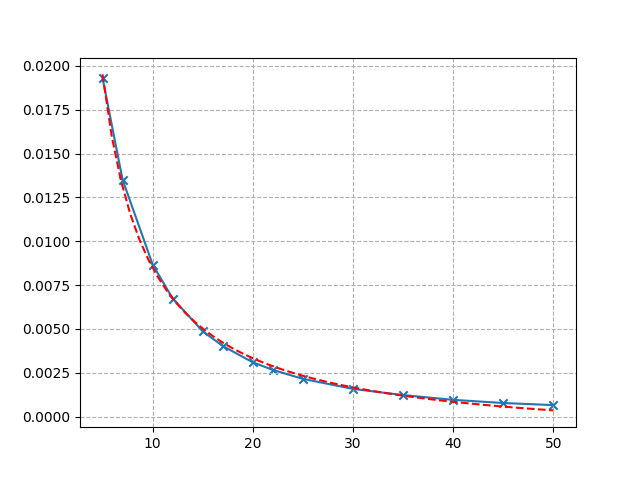
\includegraphics[width=0.5\textwidth]{Dati_sim}
\caption{Simuation}
\label{simu}
\end{figure}

 		\subsection{$^{137}\ch{Cs}$ measures}

\appendix
\chapter{137 Cesio}
\label{app_cesio}
\begin{figure}[H]
\centering
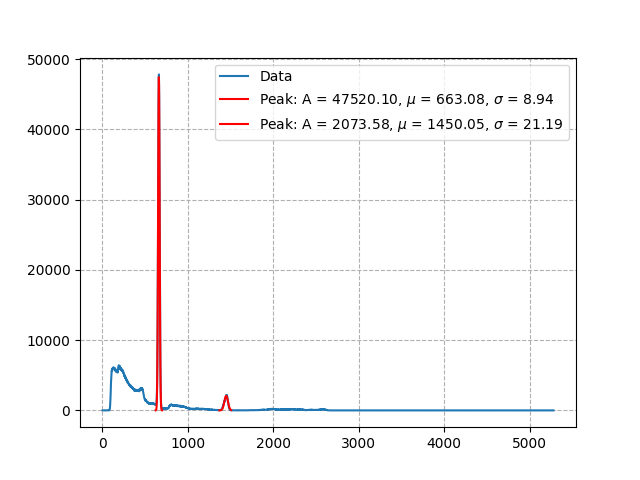
\includegraphics[width=0.3\textwidth]{cesio137_5cm}
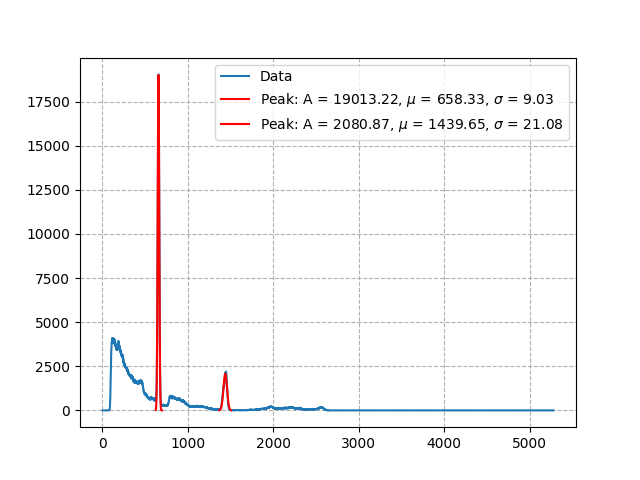
\includegraphics[width=0.3\textwidth]{cesio137_10cm}
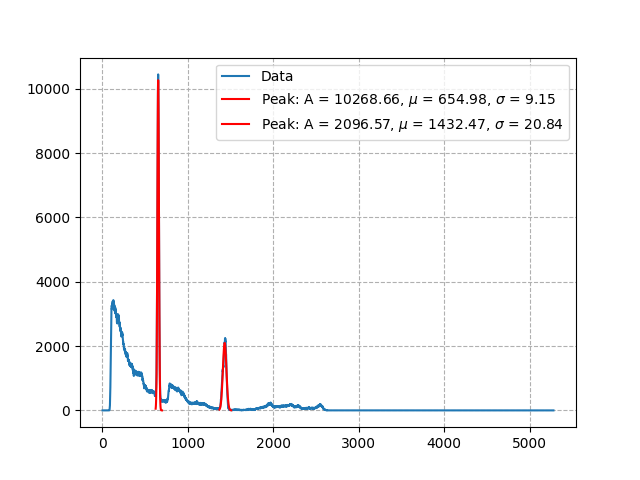
\includegraphics[width=0.3\textwidth]{cesio137_15cm}
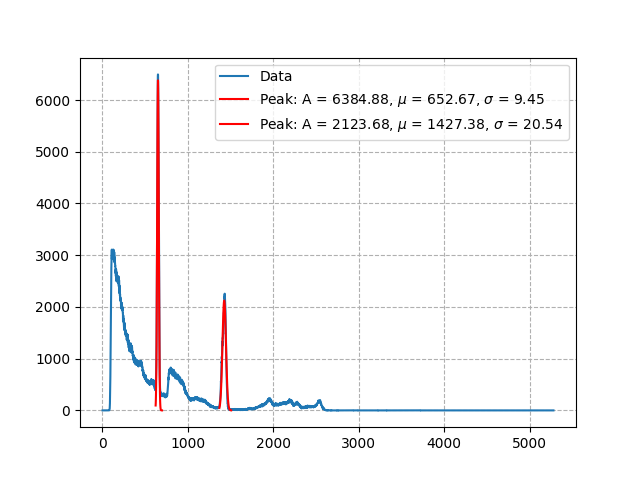
\includegraphics[width=0.3\textwidth]{cesio137_20cm}
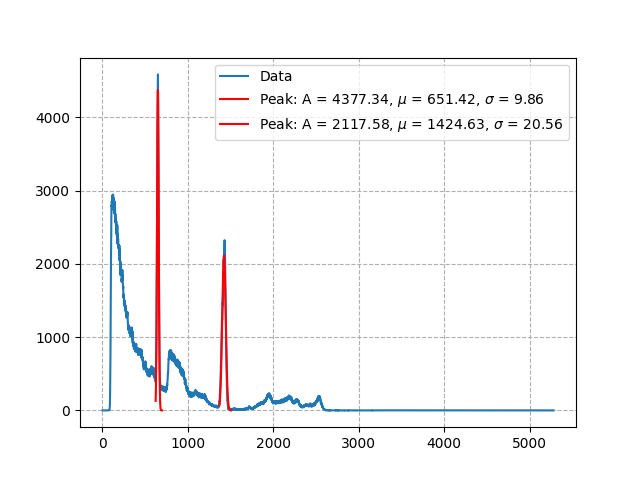
\includegraphics[width=0.3\textwidth]{cesio137_25cm}
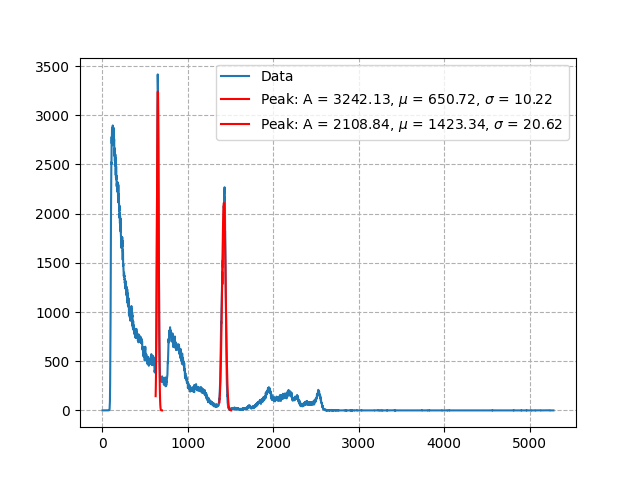
\includegraphics[width=0.3\textwidth]{cesio137_30cm}
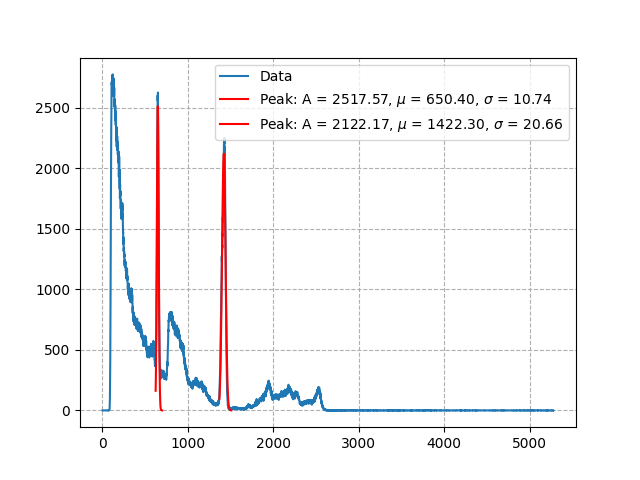
\includegraphics[width=0.3\textwidth]{cesio137_35cm}
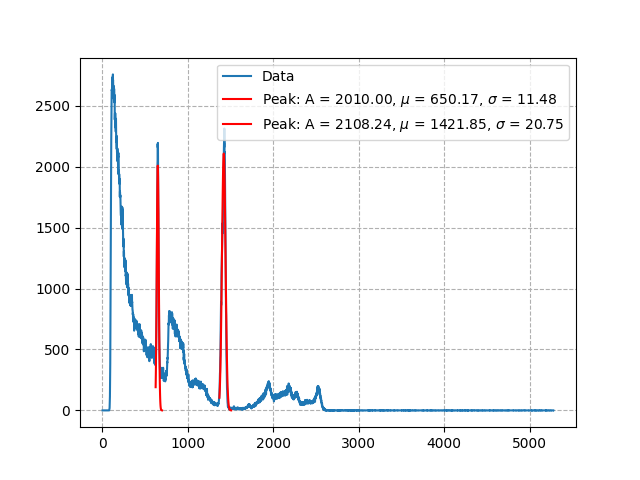
\includegraphics[width=0.3\textwidth]{cesio137_40cm}
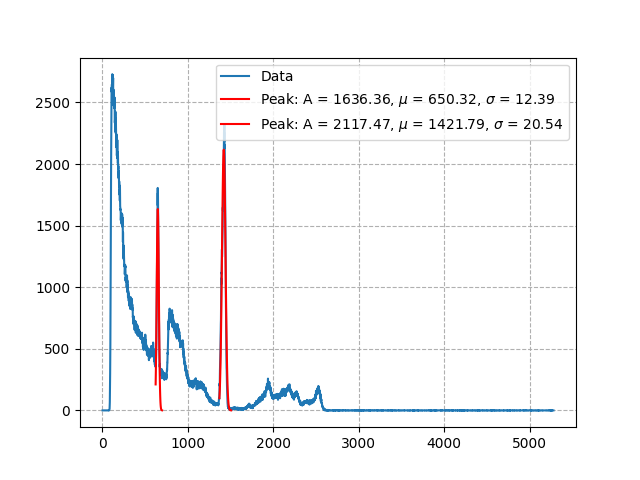
\includegraphics[width=0.3\textwidth]{cesio137_45cm}
\end{figure}

\chapter{Parameter}
$^{138}\ch{La}$ half-life: $\tau_{1/2}=1.02\cdot10^{11}$ years\\
$^{137}\ch{Cs}$ half-life: $\tau_{1/2}=30.08$ years\\
Relative efficiency: $\epsilon=19\%$\\
Branching ratio: $BR=65.2\%$\\
Isotopic abundance: $AI=0.08881\%$\\
Avogadro's number: $N_{A}=6.023\cdot10^{23}$\\
$\ch{LaBr3}$ molar mass: $mm_{\ch{LaBr3}}=378.61$\\
$\ch{CeBr3}$ molar mass: $mm_{\ch{CeBr3}}=379.82$\\
$\ch{LaBr3}$ density: $\rho_{\ch{LaBr3}}=5.06 g/cm^{3}$\\
$\ch{CeBr3}$ density: $\rho_{\ch{CeBr3}}=5.1 g/cm^{3}$\\
Time: $t=1200 s$\\
$^{137}\ch{Cs}$ activity in 2015: $A_{0}=41.3 kBq$\\

\chapter{Error propagation}
\begin{equation}
\sigma^{2}_{F}=\sum^{N}_{i=1}\left(\frac{\delta F}{\delta x_{i}}\right)^{2}\sigma^{2}_{i} + 2\sum_{i<j}\frac{\delta F}{\delta x_{i}}\frac{\delta F}{\delta x_{j}}\rho_{ij}\sigma_{i}\sigma{j}
\end{equation}
$\sigma_{i}$ represents the measurement error for the i-quantity, while $\rho_{ij}$ is the correlation coefficient.

\end{document}